\begin{frame}
  \frametitle{Proyecciones de Deuda Neta del GNC}
  \begin{center}
    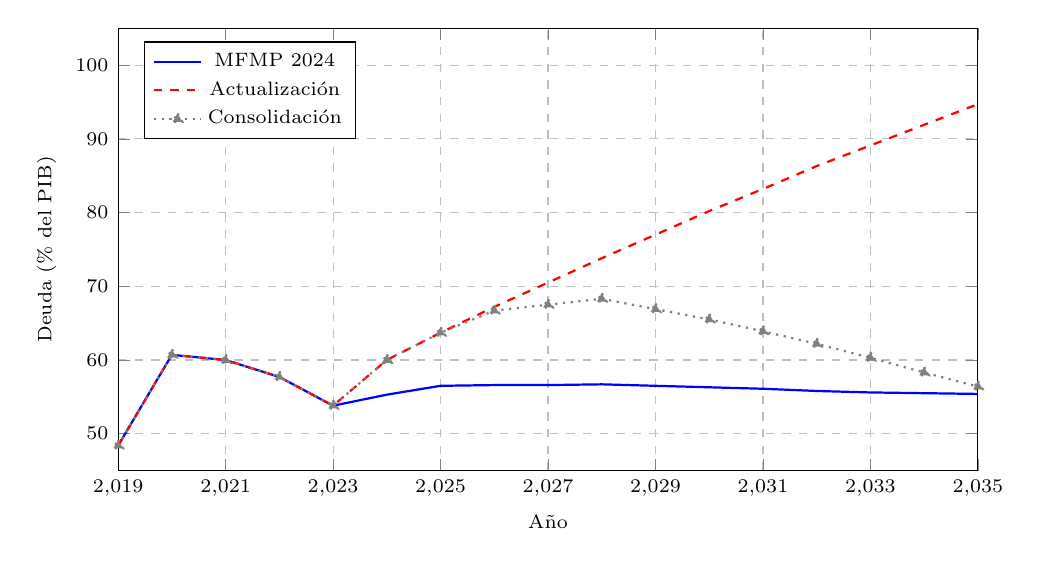
\begin{tikzpicture}
    \begin{axis}[
        width=12.5cm, height=7.2cm,
        xlabel={Año},
        ylabel={Deuda (\% del PIB)},
        xmin=2019, xmax=2035,
        ymin=45, ymax=105,
        xtick={2019,2021,...,2035},
        ytick={50,60,...,100},
        legend pos=north west,
        grid=major,
        grid style=dashed,
        tick label style={font=\scriptsize},
        label style={font=\scriptsize},
        legend style={font=\scriptsize}
    ]

    % Deuda MFMP 2024
    \addplot[color=blue, thick] coordinates {
        (2019,48.4) (2020,60.7) (2021,60.0) (2022,57.7) (2023,53.8) 
        (2024,55.3) (2025,56.5) (2026,56.6) (2027,56.6) (2028,56.7) 
        (2029,56.5) (2030,56.3) (2031,56.1) (2032,55.8) (2033,55.6) 
        (2034,55.5) (2035,55.4)
    };
    \addlegendentry{MFMP 2024}

    % Deuda Actualizada
    \addplot[color=red, thick, dashed] coordinates {
        (2019,48.4) (2020,60.7) (2021,60.0) (2022,57.7) (2023,53.8) 
        (2024,60.0) (2025,63.7) (2026,67.2) (2027,70.5) (2028,73.8) 
        (2029,77.0) (2030,80.2) (2031,83.2) (2032,86.3) (2033,89.1) 
        (2034,91.9) (2035,94.7)
    };
    \addlegendentry{Actualización}

    % Deuda Consolidación
    \addplot[mark=triangle*, color=gray, thick, dotted] coordinates {
        (2019,48.4) (2020,60.7) (2021,60.0) (2022,57.7) (2023,53.8) 
        (2024,60.0) (2025,63.7) (2026,66.7) (2027,67.5) (2028,68.3) 
        (2029,66.9) (2030,65.5) (2031,63.9) (2032,62.2) (2033,60.3) 
        (2034,58.3) (2035,56.4)
    };
    \addlegendentry{Consolidación}

    \end{axis}
    \end{tikzpicture}

%    \vspace{0.2cm}
%    \scriptsize\textit{Fuente: Cálculos propios con base en MFMP 2024 del Ministerio de Hacienda.}
  \end{center}
\end{frame}



\begin{frame}
  \frametitle{Proyecciones del Balance Primario del GNC}
  \begin{center}
    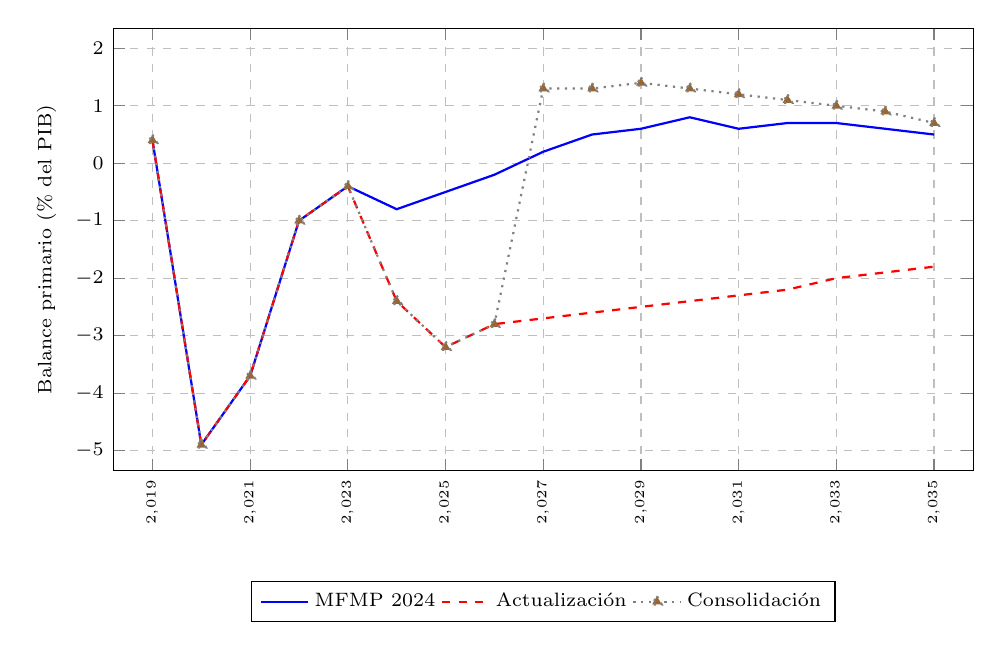
\begin{tikzpicture}
    \begin{axis}[
        width=12.5cm, % ajustado para que quepa bien
        height=7.2cm,
        ylabel={Balance primario (\% del PIB)},
        xmin=2019, xmax=2035,
        ymin=-5, ymax=2,
        xtick={2019,2021,...,2035},
        xticklabel style={rotate=90, anchor=east, font=\tiny},
        ytick={-5,-4,-3,-2,-1,0,1,2},
        yticklabel style={font=\scriptsize},
        grid=both,
        grid style=dashed,
        enlargelimits=0.05,
        tick style={thin},
        label style={font=\scriptsize},
        tick label style={font=\scriptsize},
        legend style={
            at={(0.5,-0.25)},
            anchor=north,
            font=\scriptsize,
            legend columns=3
        }
    ]

    % MFMP 2024
    \addplot+[mark=none, color=blue, thick] coordinates {
    (2019,0.4) (2020,-4.9) (2021,-3.7) (2022,-1.0) (2023,-0.4)
    (2024,-0.8) (2025,-0.5) (2026,-0.2) (2027,0.2) (2028,0.5)
    (2029,0.6) (2030,0.8) (2031,0.6) (2032,0.7) (2033,0.7) (2034,0.6) (2035,0.5)
    };
    \addlegendentry{MFMP 2024}

    % Actualización
    \addplot+[mark=none, color=red, thick, dashed] coordinates {
    (2019,0.4) (2020,-4.9) (2021,-3.7) (2022,-1.0) (2023,-0.4)
    (2024,-2.4) (2025,-3.2) (2026,-2.8) (2027,-2.7) (2028,-2.6)
    (2029,-2.5) (2030,-2.4) (2031,-2.3) (2032,-2.2) (2033,-2.0) (2034,-1.9) (2035,-1.8)
    };
    \addlegendentry{Actualización}

    % Consolidación
    \addplot+[mark=triangle*, color=gray, thick, dotted] coordinates {
    (2019,0.4) (2020,-4.9) (2021,-3.7) (2022,-1.0) (2023,-0.4)
    (2024,-2.4) (2025,-3.2) (2026,-2.8) (2027,1.3) (2028,1.3)
    (2029,1.4) (2030,1.3) (2031,1.2) (2032,1.1) (2033,1.0) (2034,0.9) (2035,0.7)
    };
    \addlegendentry{Consolidación}

    \end{axis}
    \end{tikzpicture}

%    \vspace{0.2cm}
%    \scriptsize\textit{Fuente: Elaboración propia con base en MFMP 2024, Balance del GNC y Deuda del GNC, Ministerio de Hacienda.}
  \end{center}
\end{frame}


